\chapter{Machine Learning}
\label{chp:machine_learning}

Machine learning is a way of using statistics to solve problems either by learning from a data set how what the output should be for an input or by figure out different patterns in the data. This is called supervised and unsupervised learning respectively. It is widely used in spam filtering and search engines.

\section{The Basics}
The basics for machine learning is to use to the computer to create a model from which the computer is able to predict the output or category of an input based on the values of the input. 
Machine learning most often consists of two phases, training and testing. In the training phase does the classifier model analyse the dataset given to work out how to categorize the observation and find patterns. Testing is where a new dataset is used to see how accurate the algorithm is. It is normal to divide a dataset in two for these phases, using no less than 50 percent in the training phase.
The training can be done either supervised or unsupervised. Supervised learning means the data has a label of which it is meant to be categorized as, and unsupervised use unlabeled data with the assumption that the majority of data is considered normal. In this project the data were unlabeled so the training had to be done unsupervised

\section{Anomaly Detection}
Anomaly detection, also called outlier detection, is a problem very suited for machine learning. It is a way of identify observations or data which doesn't fit an expected pattern. These observations will be referred to as anomalies or outliers in this report. Illustrated in \fref{fig:anomalyExample} is an example of anomalies in a two-dimensional data set. $N_1$ and $N_2$ is the normal areas where most of the observations are, $o_1$ and $o_2$ are anomalies and $O_3$ is an area with multiple anomalies. 

\begin{figure}
\centering
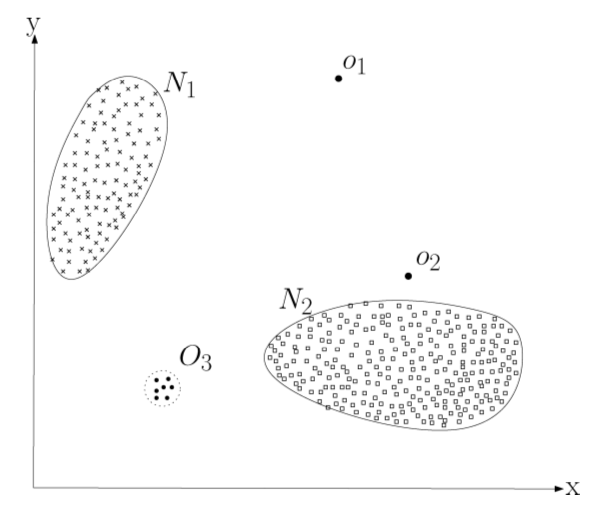
\includegraphics[scale=0.3]{figs/anomaly_example.png}
\caption{\label{fig:anomalyExample}Example of anomalies in a 2D dataset\citep{chandola2009anomaly}.}
\end{figure}



\section{Scikit-learn}
Scikit-learn was chosen as the machine learning library in this project. It is a Python library and I am most comfortable programming in Python. Alternatively could either Weka or R be used. Weka is a complete program with GUI, and has an API making it possible to integrate in a Java program. R is a special programming language which is specifically designed for statistical analysis. Scikit-learn depends on \texttt{numpy} and \texttt{scipy} to have the data in correct arrays and to do statistical analysis, and to create graphs is it necessary to use \texttt{matplotlib}. These do not follow in the regular installation of scikit-learn, and will have to be install on its own. 

\subsection{Models}
\glspl{svm} is general terms for models that use supervised learning to analyse and recognize patterns in the data given as a training set. The problem must be binary, which means each point must belong to one of two categories. \gls{ocsvm} is a unsupervised \gls{svm} model, which is used used to solve outlier detection problems. In this project that was needed since the data was not labeled. Elliptical envelope was also used to see the difference between machine learning models. It is a covariance model, and is used to calculate a \gls{mcd}. \gls{mcd} is a function that tries to find a proportion value of the correct observations which is then used to weight the observation to give a better representation \cite{scikit-learn}.